\chapter{کارهای پیشین}
در این فصل کارهای پیشین انجام‌شده روی مسئله به تفصیل توضیح داده می‌شود.
\section{تشخیص تروا‌های سخت‌افزاری}
واگذار کردن طراحی و ساخت تراشه‌ها به شرکتها و کارخانجات خارجی در کنار افزایش استفاده از هسته‌های IP دیگر شرکتها و ابزارهای خودکار سازی طراحی که سایرین طراحی کرده‌اند، موجب شده‌است تا مدارات مجتمع نسبت به حملات تروا‌های سخت‌افزاری آسیب پذیرتر شوند. در بخش گذشته انواع تروا‌های سخت‌افزاری معرفی شدند. در این بخش انواع روش‌های تشخیص تروا را مرور می‌کنیم. روش‌های مختلف شرح داده می‌شوند و براساس قابلیت‌ها و محدودیت‌هایشان مقایسه می‌شوند. متاسفانه استفاده از روش‌های آزمون مدارات که در گذشته ارائه شده‌اند، برای تشخیص تروا مفید نیست. چرا که این روش‌ها در پی تشخیص عملکرد نادرست ناشی از اشکالات فرآیند ساخت هستند و عملکردهای اضافی ناشی از تروا را تشخیص نمی‌دهند. تروا‌هایی که به صورت هوشمندانه در مدار اضافه می‌شوند، معمولاً به ندرت تحریک می‌شوند و بنابراین تشخیص آنها سخت است. همچنین ممکن است برخی تروا‌ها هیچ اثری بر عملکرد عادی مدار نداشته باشند و برای مثال تنها اطلاعاتی را به خارج از مدار منتقل کنند
$\cite{lin2009trojan}$. 
تولید بردارهای آزمونی که تمام نقاط مدار را به طور کامل بیازمایند، واقعاً شدنی نیست. مخصوصاً اگر تروا از نوع مدار ترتیبی باشد که با رخداد ترتیب خاصی از وقایع نادر فعال می‌شود. از سوی دیگر می‌توان تروا‌ها را براساس اثر جانبی که بر توان مصرفی یا تاخیر می گذارند شناسایی کرد. با این روش دیگر نیازی به فعالسازی کامل تروا و مشاهده اثر آن بر خروجی مدار نیست. از طرفی دقت چنین روش‌هایی برای تشخیص تروا‌های کوچک، به علت اثر سوئی که تغییرات فرآیند و نویز بر تغییر توان یا تاخیر دارد، خیلی بالا نخواهد بود. 
استفاده از روش آزمون عملکردی و تحلیل اثرات جانبی برای تشخیص همه تروا‌ها کافی نیست. بنابراین می‌توان از روش نظارت حین اجرا برای بهبود سطح اطمینان از وجود تروا، استفاده کرد. برای مثال تروای که اطلاعاتی را از یک تراشه رمزنگاری از طریق کانال بی سیم نشت می‌دهد، ممکن است توان گذرای زیادی را در برهه‌ای از زمان که بنا نیست ارتباطاتی انجام شود، مصرف کند. در این حالت استفاده از روش‌های نظارت در حین اجرا، مناسبتر است.
ارزیابی میزان قابلیت اعتماد در هسته‌های IP به علت عدم وجود مدل مرجعی که با آن مقایسه شوند، مشکل تر است. در این موارد می‌توان از آزمون‌های عملکردی استفاده کرد. این روش تنها زمانی موثر خواهد بود که اطلاعاتی درباره شرایط تحریک تروا و اثر تروا داشته باشیم. روش دیگر استفاده از اعتبار سنجی صوری است. 
روش‌های تشخیص تروای که تا کنون ارائه شده‌اند قابلیت‌ها و محدودیت‌های خاص خود را دارند. اما تا کنون روشی کامل برای تشخیص تمامی انواع تروا‌ها با درجه اطمینان بالا ارائه نشده‌است. یک راه حل برای بالا بردن درجه اطمینان، ترکیب روش‌های مختلف با یکدیگر است. در ادامه ابتدا به دسته‌بندی روش‌های تشخیص تروا‌های سخت‌افزاری می پردازیم و بعد از بررسی چالش‌های پیش رو در روش‌های تشخیص تروا، مروری کلی بر انواع روش‌های ارائه شده داریم.
\section{دسته‌بندی روش‌های تشخیص تروا}
\begin{figure}
	\begin{center}
		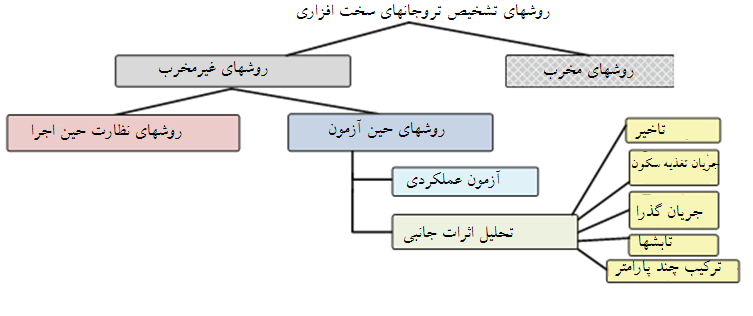
\includegraphics[scale=.8]{figs/fig1-4.png}
		\caption[دسته‌بندی روش‌های تشخیص ترواهای سخت‌افزاری]
		{دسته‌بندی روش‌های تشخیص ترواهای سخت‌افزاری
			$\cite{rai2009performance}$}
		\label{fig1-4}
	\end{center}
\end{figure} 

در شکل \ref{fig1-4} نمودار دسته‌بندی روش‌های تشخیص تروا ارائه شده‌است. این روش‌ها به دو دسته عمده مخرب و غیرمخرب دسته‌بندی می‌شوند. در روش‌های مخرب لازم است تراشه‌های ساخته شده با روش CMP\footnote{\lr{Chemical-Mechanical Planarisation}} لایه برداری شوند تا تصاویر لایه به لایه با استفاده از میکروسکوپ الکترونی پویشی، گرفته شود. در این روش، رویکرد مهندسی معکوس بالا به پایین استفاده می‌شود. این روش‌ها به شدت گران و زمان بر(چندین ماه
$\cite{torrance2007reverse}$
) هستند. این روش برای ارزیابی تک تک تراشه‌ها اصلا مقرون به صرفه نیست. تنها مورد استفاده از این روش بدست آوردن یک مدل مرجع برای حذف اثر تغییرات فرآیند در روش‌های دیگر تشخیص تروا است. 
روش‌های غیرمخرب را می‌توان به دو دسته رویکردهای نظارت حین اجرا و رویکردهای زمان آزمون تقسیم کرد.شایان ذکر است که روش‌های نظارت حین اجرا معمولاً روش‌های هجومی هستند که بعضی از روش‌های طراحی برای امنیت \footnote{\lr{Design for Security}}DfS از آنها استفاده می‌کنند. این روش‌ها می‌توانند از افزونگی موجود در مدار استفاده کنند. به این نحو که از یک هسته با قابلیت پیکربندی مجدد در سیستم‌های چندهسته‌ای برای ممانعت از اثرگذاری مدار دارای تروا بهره گرفته می‌شود تا با وجود تروا، قابلیت اطمینان سیستم تضمین شود. دسته‌ای دیگر از روش‌ها برای سیستم‌های با ماموریت بحرانی، روش‌های خود تخریبی هستند که به صورت خارجی توسط کاربر یا داخلی توسط ناظر تروا، فعال می‌شوند. 
روش‌های حین آزمون نیز می‌توانند از مدارات DfS کمک بگیرند. این مدارات می‌توانند حساسیت روش‌های تشخیص تروا را افزایش دهند و یا پوشش دهی تشخیص تروا‌ها را بیشتر کنند. اگر سیگنال فعال کننده حالت آزمون، به راحتی قابل تشخیص باشد، طراح تروا می‌تواند ترتیبی دهد که با فعال شدن این سیگنال تروا غیر فعال شود. روش‌های حین آزمون را می‌توان به دو دسته کوچکتر روش‌های مبتنی بر آزمون عملکردی و روش‌های مبتنی بر تحلیل اثرات جانبی، تقسیم کرد.
روش‌های آزمون عملکردی 
$\cite{li2008speed,rai2009performance}$
بر تولید بردارهای آزمون و اعمال آنها برای فعالسازی تروا و مشاهده نتایج مخرب آن در خروجی‌های مدار متمرکز هستند. روش کار مشابه آزمون‌های لازم برای یافتن اشکالات \footnote{\lr{stuck-at}} است. اما مدل‌های تروا بسیار متفاوت با مدل‌های اشکال هستند. تروا‌ها هوشمندانه در مدار درج می‌شوند و در مواقع نادری تحریک می‌شوند. تعداد کل تروا‌های ممکن از یک نوع و اندازه خاص، تابع نمایی از تعداد دروازه‌های منطقی مدار است. همچنین در مورد تروا‌های ترتیبی که باید رشته ای از رخدادها به ترتیب رخ دهد تا آن را فعال کند، ممکن است در طول زمان آزمون نتیجه تروا مشاهده نگردد. بنابراین روش‌های تشخیص اشکال را نمی‌توان برای تشخیص تروا به کار گرفت.
از سویی دیگر روش‌های تحلیل اثرات جانبی مبتنی بر این حقیقت هستند که هر نوع درج مدارات مخرب در تراشه بایستی به صورت تغییر بعضی از پارامترها در سیگنال‌های جانبی مثل جریان نشتی، جریان تغذیه سکون $\cite{aarestad2010detecting,alkabani2009consistency,potkonjak2009hardware}$، توان پویا $\cite{agrawal2007trojan,banga2008region,banga2009novel,salmani2010layout,du2010self}$، مشخصات تاخیری $\cite{jin2008hardware,li2008speed}$، تابشهای الکترومغناطیس ناشی از فعالیت سیگنال‌ها $\cite{agrawal2007trojan}$ یا ترکیبی از موارد پیش گفته $\cite{narasimhan2010multiple,tehranipoor2012introduction}$ ، خودش را نشان دهد.
روش‌های بسیاری مبتنی بر رویکرد تحلیل اثرات جانبی ارائه شده‌است. مشکل اصلی آنها این است که نسبت به نویز محیط و تغییرات فرآیند حساس هستند. بنابراین مساله تشخیص تروا به عنوان یک رویداد آماری با هدف بیشینه کردن احتمال تشخیص و کمینه کردن احتمال تشخیص غلط مدنظر قرار می‌گیرد. تولید بردارهای آزمون می‌تواند نقش مهمی در روش‌های تحلیل اثرات جانبی بازی کند. بدین صورت که حساسیت تشخیص تروا را خصوصاً در مورد تروا‌های کوچک در مدارات SoC بزرگ، افزایش دهد. معمولاً تروا در فضاهای خالی layout\footnote{چینش} درج می‌شود و با اهداف خرابکارانه این مدارات به یکدیگر سیم بندی می‌شوند. با تمام این اوصاف، رویکرد تحلیل اثرات جانبی نسبت به رویکرد آزمون منطقی این مزیت را دارد که لازم نیست برای تشخیص تروا آن را فعال کنیم. بنابراین این دسته روش‌ها برای تشخیص تروا‌هایی موثر هستند که موجب تغییر عملکرد مدار نمی‌شوند و هدفشان افشای اطلاعات محرمانه از طریق سیگنال‌های جانبی است.
\subsection{رویکردهای مبتنی بر آزمون منطقی}
از آنجا که تشخیص تروا با آزمون عملکردی متفاوت با آزمون‌های رایج برای یافتن اشکالات مدار است، روش‌های آماری تولید بردار برای تشخیص تروا بسیار مناسبتر هستند. در $\cite{jha2008randomization}$ روش تصادفی برای مقایسه احتمالاتی عملکرد مدار با مدل مرجع ارائه شده‌است. هر گونه تفاوت در عملکرد دو مدار برای تشخیص حضور تروا استفاده می‌شود و بردار ورودی که موجب این اختلاف شده‌است، اثر انگشت آن تروای خاص نامیده می‌شود. در این روش هیچ مدل خاصی برای تروا به منظور تولید بردارهای آزمون مدنظر قرار نگرفته‌است و صرفاً بر یافتن تساوی عملکرد دو مدار متمرکز است. این رویکرد برای تایید اعتبار هسته‌های IP نیز کاربرد دارد.
در $\cite{chakraborty2009mero,borkar2003parameter}$ یک روش تولید بردار آماری برای تشخیص تروا ارائه شده‌است که MERO نام دارد. در این روش مجموعه بهینه‌ای از بردارهای آزمون تولید می‌شود که هر گره با فعالیت کم در مدار را می‌تواند چندین بار به مقدار نادرش مقدار دهی کند. این روش شبیه روش آزمون N-Detect است $\cite{pomeranz2004measure}$. تعیین نادر بودن رخداد و تعداد گره‌های تحریک تروا و ماهیت تروا(ترکیبی یا ترتیبی) همگی متغیرهای ورودی به الگوریتم هستند. با فعالسازی تک به تک گره‌های نادر، احتمال تحریک تروای که با ترکیب نادری از این گره‌ها فعال می‌شود، بیشتر می‌شود. با این روش تحریک تروا از تشخیص آن ساده‌تر می‌شود. چراکه معمولاً مدار بار مربوط به تروا از مشاهده‌پذیری پایینی برخوردار است. با استفاده از دو معیار پوشش تحریک و پوشش تروا این الگوریتم ارزیابی شده‌است. هرچه تعداد دفعات مقداردهی به گره‌های نادر بیشتر شود، این دو معیار بهبود خواهد یافت. با این همه اینکار باعث افزایش زمان آزمون خواهد شد. همچنین در این روش برای مدارات ترتیبی، از فلیپ فلاپ‌های پویش برای کاهش مدت آزمون و افزایش پوشش‌دهی، استفاده شده‌است.
علاوه بر روش‌های بالا، می‌توان از روش‌های DfS نیز برای افزایش قابلیت آزمون پذیری مدارات بزرگ با رویکرد بهبود کنترل‌پذیری و مشاهده‌پذیری گره‌هایی که محتمل است گره تحریک تروا یا گره بار باشند، استفاده کرد. با افزودن یک ماشین حالات کنترلی که تشخیص آن مشکل باشد، ماژولهای مختلف داخل مدار را می‌توان به صورت انتخابی آزمود. با اعمال رشته خاصی از ورودی‌ها، هر ماژول به وضعیت خاصی که وضعیتِ شفاف $\cite{chakraborty2008demand}$ نام دارد، وارد می‌شود. در این وضعیت، سایر ماژولها به نحوی از چرخه عملکرد خارج می‌شوند و وجود یا عدم وجود تروا در این ماژول خاص بررسی می‌شود.
\subsection{روش‌های مبتنی بر تحلیل اثرات جانبی}
تمامی روش‌های مبتنی بر تحلیل اثرات جانبی، بر مشاهده اثر تروا بر یک پارامتر فیزیکی مثل جریان تغذیه(گذرا یا دائمی)، توان مصرفی، یا تاخیر مسیرها، استوار هستند. مزیت استفاده از این روش‌ها در این است که حتی اگر مدار تروا در طول زمان آزمون، تاثیر قابل مشاهده‌ای در خروجی نگذارد، حضور مدار اضافه ناشی از تروا در پارامترهای جانبی قابل تشخیص است. مساله اصلی در این روش‌ها این است که در تکنولوژی‌های ابعاد نانو، اثرات جانبی با تغییر فرآیند به شدت تغییر می‌کنند و این امر در کنار نویز اندازه‌گیری، تشخیص تروا را بخصوص اگر مداری کوچک باشد، مشکل می‌کند. در ادامه انواع سیگنال‌هایی که در این روش‌ها به عنوان اثر جانبی از آنها استفاده می شود، مرور می‌شود و روش‌هایی که از این سیگنال‌ها استفاده کرده‌اند، شرح داده خواهد شد.
\\
\footnote{\lr{Integrated Dual Disorder Quiescent }}IDDQ روشن است که جریانی که از منبع تغذیه کشیده می‌شود، با افزودن مدارات اضافه به مدار اصلی، تغییر خواهد کرد. هر دروازه منطقی اضافه باعث افزایش جریان نشتی می‌شود و اندازه‌گیری مجموع این جریان‌های اضافه، تشخیص تروا را تسهیل می‌کند. البته این افزایش ناشی از جریان نشتی دربرابر جریانی که یک مدار بزرگ چند میلیون گیتی از تغذیه می‌کشد، بسیار ناچیز است و تشخیص آن دشوار است. برای بالابردن احتمال تشخیص تروا، می‌توان جریان را از چندین پایه تغذیه اندازه‌گیری نمود. به این روش، روش مبتنی بر ناحیه گفته می‌شود.
\\
IDDT\footnote{\lr{Integrated Dual Disorder Treatment}}
جریان گذرای منبع تغذیه که نشانگر توان پویای ناشی از فعالیت سوئیچینگ مدار است، نیز از طریق پایه‌های تغذیه قابل
اندازه‌گیری است. این جریان بیانگر تعداد دروازه‌های منطقی است که با اعمال بردار خاصی به ورودی، خروجی‌شان تغییر می‌کند. بنابراین اعمال بردارهای ورودی و اندازه‌گیری جریان گذرا می‌تواند حساسیت روش‌های تشخیص تروا را به وجود تروا افزایش دهد. همانطور که در\\
شکل
\ref{fig4-4}
نشان داده شده‌است، حساسیت در تشخیص تروا با کاهش اندازه تروا، کاهش می یابد. اما با انتخاب مناسب بردارهای ورودی، این حساسیت قابل افزایش است. این مساله مقیاس پذیری این روش را بهبود می بخشد.
\begin{figure}
	\begin{center}
		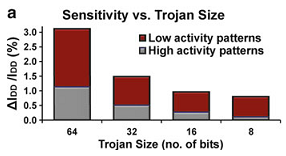
\includegraphics[scale=1]{figs/fig4-4.png}
		\caption[اثر اندازه تروا بر جریان نشتی و جریان گذرای تغذیه]
		{اثر اندازه تروا بر جریان نشتی و جریان گذرای تغذیه $\cite{chakraborty2008demand}$}
		\label{fig4-4}
	\end{center}
\end{figure} 
تاخیر: پارامتر سومی که می‌تواند در تشخیص تروا استفاده شود، تاخیر مسیرهاست. اگر تروا در مسیری باشد که تاخیرش اندازه‌گیری می‌شود، بسته به تعداد دروازه‌های منطقی که در مسیر اضافه شده‌است، تاخیر مسیر را افزایش خواهد داد. حتی اگر بردار ورودی اعمال شده، تروا را بطور کامل فعال نکند، مقداری خازن بار به گره اضافه می‌کند و بنابراین باعث افزایش تاخیر می‌شود. البته اگر تاخیر مسیر اصلی خیلی زیاد باشد، این تغییرات کوچک ممکن است به چشم نیاید و تغییرات ناشی از تغییر فرآیند، آن را بپوشاند. لازم به ذکر است که تنها تاخیر مسیرهایی که از ورودی‌ها شروع شده و به خروجی‌ها ختم می‌شوند، قابل اندازه‌گیری است. بنابراین برای مدارات ترتیبی اگر از پویش کامل استفاده نشود، زمان زیادی باید صرف اندازه‌گیری همه مسیرها شود.
تشعشعات الکترومغناطیس: تابشهای الکترومغناطیس ناشی از فعالیت سوئیچینگ دروازه‌های منطقی مختلف، می‌تواند جهت تشخیص وجود مدار اضافی ناشی از تروا مورد مشاهده قرار گیرد. روش‌هایی که از این رویکرد استفاده می‌کنند در همان دسته‌ای قرار می‌گیرند که روش‌های استفاده کننده از جریان گذرا هستند.
روش‌های موجود سعی می‌کنند با نرمال سازی یا تخمین گوشه‌های فرآیند، اثر تغییر فرآیند را بر تغییر پارامتر اندازه‌گیری شده، مدل کنند و بدین ترتیب اثر آنها را حذف نمایند. با استفاده از روش مبتنی بر ناحیه، که از چندین پایه تغذیه جداگانه اندازه‌گیری را انجام می‌دهد، نویزهایی که متناسب با مقدار اندازه‌گیری شده هستند ( مثل نویز تغییر فرآیند) کاهش می یابد. می‌توان از پردازش سیگنال آماری برای محاسبه نویز فرآیند و کاهش اثر آن بر مقدار اندازه‌گیری شده ‌استفاده کرد.
روش اثرانگشت برداری از مدار $\cite{agrawal2007trojan}$ برای کالیبراسیون نویز فرآیند استفاده می‌شود و برای تشخیص بخش‌هایی از گزارش توان مصرفی که حضور تروا را نشان می‌دهد، نیز استفاده شده‌است. با استفاده از این روش می‌توان تروا‌هایی با ابعاد 0.01 درصد ابعاد مدار را شناسایی کرد. 
برای افزایش احتمال فعال شدن تروا با اعمال بردارهای آزمون به ورودی‌ها، روش تولید بردار آزمون مناسب باید انتخاب شود. برای مدارات ترتیبی بزرگ، روش فعالسازی مبتنی بر ناحیه مدار برای افزایش حساسیت روش‌های مبتنی بر اثرات جانبی موثر خواهد بود. مدار را می‌توان به بخش‌هایی که از نظر عملکردی از هم جدا هستند، تقسیم‌بندی کرد یا به صورت ساختاری به نحوی تقسیم‌بندی کرد که همپوشانی نواحی کمینه باشد. بعد از آن بردارهای آزمونی که به صورت هدایت شده تولید شده‌اند، برای افزایش فعالیت سوئیچینگ در ناحیه مورد نظر و با هدف کاهش فعالیت در سایر مدار، اعمال می‌شوند. بنابراین حساسیت روش تشخیص تروا در ناحیه فعال، افزایش می یابد. کارایی این روش در $\cite{banga2008region}$ نشان داده شده‌است. روش بردار پایدار شده نیز برای افزایش بیشتر حساسیت در تشخیص تروا استفاده می‌شود. در این روش بردارهای اعمالی به ورودی‌ها برای چندین پالس ساعت ثابت نگهداشته می‌شوند تا تنها فعالیت ناشی از تغییر مقادیر عناصر حافظه ای وجود داشته باشد و بدین ترتیب جریان مدار اصلی تا حدامکان کاهش یابد. این روش در $\cite{banga2009novel}$ شرح داده شده‌است و برای بزرگ‌نمایی تفاوت بین توان مصرفی مدار اصلی و مدار دارای تروا استفاده شده‌است.
روش دیگر مبتنی بر ناحیه برای کالیبراسیون نویز فرآیند در قالب شبکه تغذیه روی تراشه در 
$\cite{rad2010sensitivity, aarestad2010detecting}$
ارائه شده‌است. نوعاً مدارات، یک شبکه تغذیه توزیع شده در لایه‌های فلزی بالا دارند که شامل برآمدگی‌هایی است که به پایه‌های مختلف تراشه متصل است. از بیرون تراشه و در سطح بورد، این پایه‌ها می‌توانند به یک منبع تغذیه یکپارچه متصل شده باشند. اندازه‌گیری جریان از پایه‌های مختلف تغذیه به ازای ورودی‌های مختلف، و در ادامه انتگرال‌گیری روی جریان، می‌تواند برای اندازه‌گیری انتقال بار الکتریکی در طول فعالیت سوئیچینگ به کار رود. هر مداری که دارای تروا باشد، بار بیشتری در واحد زمان جمع می‌کند. چراکه نسبت به مدار بدون تروا فعالیت سوئیچینگ بیشتری دارد. این اختلاف بار را با انتگرال‌گیری از جریان می‌توان تشخیص داد. همچنین از آنجا که اندازه‌گیری جریان از پایه‌های مختلف انجام می‌شود، موقعیت تروا نیز قابل تخمین است. شکل \ref{fig5-4} نحوه اعمال این روش را نشان می‌دهد.
\begin{figure}
	\begin{center}
		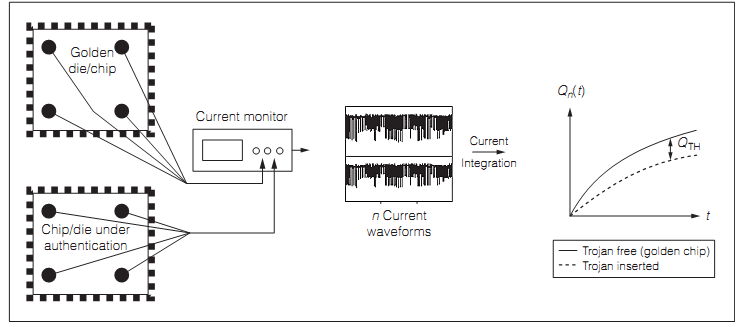
\includegraphics[scale=0.8]{figs/fig5-4.png}
		\caption[نحوه اعمال روش اندازه‌گیری جریان و بار به صورت محلی شده]
		{نحوه اعمال روش اندازه‌گیری جریان و بار به صورت محلی شده $\cite{aarestad2010detecting}$}
		\label{fig5-4}
	\end{center}
\end{figure} 
روش‌های مختلف کالیبراسیون برای حذف تغییرات مقاومتی در پایه‌های تغذیه و حذف تغییرات فرآیند درون تراشه و بین تراشه قابل استفاده است. یک مدار کالیبراسیون شامل یک ترانزیستور است که بین پایه تغذیه و زمین وصل می‌شود و می‌تواند با استفاده از سیگنال کنترلی از یک فلیپ فلاپ، خاموش یا روشن شود. تکنیک ارائه شده در این مقاله می‌تواند 50 درصد تروا‌های فعال شده و 30 درصد تروا‌های غیرفعال را تشخیص دهد. برای افزایش احتمال فعال شدن سیگنال‌های نادر، از فلیپ فلاپ‌های پویش استفاده شده‌است.
یک روش تغییر ترتیب سلولهای پویش آگاه به چینش $\cite{salmani2010layout}$ می‌تواند کنترل‌پذیری سوئیچینگ در نواحی خاص را افزایش دهد. این روش احتمال سوئیچینگ مدارات تروا را افزایش می‌دهد و در نتیجه موجب افزایش احتمال تشخیص تروا می گردد.
اندازه‌گیری تاخیر مسیرها در پایه‌های خروجی برای مجموعه‌ای از بردارهای آزمون، می‌تواند برای تشخیص حضور تروا مورد استفاده قرار گیرد. در $\cite{jin2008hardware}$ نشان داده شده‌است که حجم چنین اطلاعاتی راجع به تاخیرها که از مسیرهای مختلف مدار بدست می آید، بخصوص برای مدارات بزرگ، می‌تواند بسیار زیاد شود. روش‌های فشرده‌سازی اطلاعات مثل روش PCA\footnote{\lr{Principal Component Analysis}} را می‌توان برای کاهش ابعاد این اطلاعات بکار برد. این نقاط داده‌ای کاهش یافته را اثرانگشت تاخیر مسیر می‌نامند.
روش سریع مشخصه‌سازی تاخیر $\cite{li2008speed}$ ثبات‌های سایه را بهمراه مقایسه کننده درون تراشه قرار می‌دهد تا تاخیر مسیرهای داخلی ثبات تا ثبات را بیابد. این روش DfS از افزایش انحراف منفی کلاک ثبات سایه نسبت به کلاک عملیاتی سیستم استفاده می‌کند و نتیجه مقایسه را به ازای یک سری ورودی، ذخیره می‌کند تا توزیع تاخیر را بیابد. 
روش دیگر برای مشاهده اثر تروا بر تاخیر مسیرهای داخلی، این است که مسیرها را به صورت نوسانگرهای حلقوی  
$\cite{rajendran2011design,zhang2013detection}$
پیکربندی کنیم. با درج تروا در این مسیرها، تاخیر مسیر، به علت تغییر مقاومت و یا بخاطر همشنوایی بین سیم‌ها، تغییر خواهد کرد. فرکانس این نوسانگرها با استفاده از شمارنده‌های روی تراشه محاسبه می‌شود. مساله اصلی در این روش حذف اثر تغییر فرآیند و تغییرات محیطی است. البته طراح تروا ممکن است به نحوی تروا را اضافه کند که اثری بر فرکانس نوسان نگذارد یا اینکه مدارِ شمارنده فرکانس را به نحوی دچار مشکل کند. یک نوسانگر حلقوی را می‌توان به عنوان ناظر حرارتی برای کالیبراسیون تاخیر ناشی از دما نیز بکار برد. این روش باید با روش تولید بردارهای آزمون ترکیب شود تا به پوشش دهی بالا و زمان آزمون پایین دست یابیم. این روش را می‌توان در زمان اجرا نیز به کار گرفت.

در $\cite{potkonjak2009hardware}$ از هر دو پارامتر تاخیر مسیر و جریان نشتی برای پیاده‌سازی یک روش تشخیص تروا در سطح دروازه‌های منطقی استفاده شده‌است. مساله تشخیص تروا را می‌توان به صورت یک مساله برنامه نویسی خطی فرمول بندی کرد به صورتی که تغییرات فرآیند هر دروازه منطقی به صورت یک ضریب ثابت برای جریان نشتی یا تاخیرش لحاظ شود. این روش توانایی تشخیص حتی یک دروازه منطقی اضافه را دارد
\subsection{رویکردهای نظارت زمان اجرا}
تشخیص کامل تروا‌های با انواع و ابعاد مختلف در زمان آزمون تراشه از نظر عملی غیرممکن است. نظارتِ برخط محاسبات بحرانی می‌تواند سطح اعتماد به مدار را به شدت بالا ببرد. این روش‌ها می‌توانند در هنگام تشخیص موارد اشکال در مدار، تراشه را غیرفعال کنند یا آن را دور بزنند و امکان عملیات قابل اطمینان را فراهم کنند. یکی از روش‌های نظارت زمان اجرا مبتنی بر اضافه کردن مدارات با قابلیت بازپیکربندی است که به آنها DEFENSE یا طراحی برای فعالسازی امنیت $\cite{abramovici2009integrated}$ می‌گویند. چک کردن عملیاتی می‌تواند به صورت همروند با عملیات عادی سیستم انجام شود و در صورت بروز اختلاف با عملیات عادی، شمارنده‌های متناسب را تحریک می‌کند. معمولا هسته با قابلیت بازپیکربندی، عملیات مداری را که به درستی عمل نمی‌کند، پیاده‌سازی می نماید و مدار دارای مشکل غیرفعال می‌شود یا دورزده می‌شود.
یک رویکرد ترکیبی سخت‌افزاری و نرم‌افزاری برای نظارت زمان اجرا در $\cite{bloom2009support}$ ارائه شده‌است. یک ماژول ساده به نام حصار سخت‌افزاری که خارج از CPU است مدنظر قرار می‌گیرد. تروا‌هایی که در اینجا مدنظر هستند، از نوع رد خدمات می باشند. با استفاده از چک کردن دوره‌ای توسط سیستم عامل وجود یا عدم وجود تروا‌ها بررسی می‌شود. این روش تنها 2/2 درصد سربار کارایی به سیستم تحمیل می‌کند.
در $\cite{hicks2010overcoming}$ یک روش ترکیبی سخت‌افزاری/نرم‌افزاری به نام BlueChip ارائه شده‌است که شامل مولفه‌های زمان طراحی و مولفه‌های زمان اجراست. در این روش تشخیص مداراتِ بلااستفاده، با استفاده از آزمون‌های اعتبارسنجی انجام می‌شود و به عنوان مشکوک برچسب می خورند. در طول زمان اجرا مدارات مشکوک حذف می‌شوند و با یک مدار تشخیص استثنا جایگزین می‌شوند. با این کار مدار می‌تواند عملیات خود را بدون مشکل انجام دهد. این روش برای از بین بردن اثر تروا‌های سخت‌افزاری است که اهدافی شبیه تروا‌های نرم‌افزاری دارند. این تروا‌ها هدفهای مختلفی دارند. از جمله افزایش امتیاز یک برنامه از حالت کاربر معمولی به حالت فوق کاربر، تخصیص دسترسی به حافظه محدود شده یا شروع حملات DoS که شبیه به فراهم کردن امکان اجرای کد مخرب است.
در مورد پردازنده‌ها‌‌ی چندهسته‌ای می‌توان یک روش زمان اجرای خودزمانبند پیاده‌سازی نمود $\cite{mcintyre2009dynamic}$ که به وسیله آن، نرم‌افزاری‌ها‌‌یی با عملیات مشابه روی چندین هسته اجرا می‌شوند. خروجی‌های هسته‌های مختلف با یکدیگر مقایسه می‌شود تا به صورت پویا سطح اطمینان تک تک هسته‌ها چک شود.
\subsection{روش‌های طراحی مطمئن}
برای بهبود کارایی روش‌های تشخیص تروا و رفع محدودیت‌های آنها، روش‌های متعددی توسط محققان امنیت سخت‌افزاری ارائه شده‌است که هدف آنها تغییر روال طراحی کنونی است. به این روش‌ها، روش‌های طراحی برای اطمینان سخت‌افزاری می گویند $\cite{tehranipoor2010survey}$. هدف از این روش‌های بازدارنده تروا، این است که مانع درج تروا شوند و یا تشخیص تروا‌ها را تسهیل کنند. برخلاف روش‌های تشخیص تروا که روش‌های منفعلانه هستند، روش‌های طراحی مطمئن، روش‌هایی فعال هستند. یعنی ساختار مدار را به نحوی تغییر می‌دهند تا مانع از درج تروا شوند. برای رسیدن به این هدف، چرخه طراحی مدارات مجتمع باید دستخوش تغییر شود.
اکثر روش‌های بازدارنده از تروا، با هدف تسهیل در تشخیص تروا با استفاده از روش‌های تحلیل اثرات جانبی ارائه شده‌اند. از این پس به این روش‌ها، روش‌های مبتنی بر اثرانگشت اثرات جانبی گفته می‌شود. بعضی از این روش‌ها صرفاً امکاناتی برای اندازه‌گیری پارامترهای جانبی فراهم می‌کنند ولی برخی دیگر مقادیر اندازه‌گیری شده را با مقادیر آستانه‌ای که از قبل تعریف شده‌اند، مقایسه می‌کنند. سربار طراحی، عمده ترین چالش این روش‌هاست. چراکه مدارات اندازه‌گیری و مقایسه، به نوبه خود می‌توانند پیچیده باشند و بخش زیادی از مساحت تراشه را اشغال کنند. بر همین اساس اکثر روش‌های بازدارنده از تروا برای اندازه‌گیری و مقایسه تاخیرها استفاده می‌شوند. چرا که مدارات اندازه‌گیری تاخیر نسبتاً سربار مساحت کمتری دارند.
سایر روش‌ها بر این فرض استوار هستند که طراحان تروا تنها از رخدادهای نادر برای تحریک تروا استفاده می‌کنند. این روش‌ها سعی دارند با افزایش احتمال فعال شدن کامل تروا‌ها در طول فاز آزمون، روش‌های آزمون ساختاری/عملکردی را بهبود دهند. از میان این روش‌ها، روش مبهم سازی $\cite{chakraborty2009security}$ به نوعی مدار را پنهان می‌کند تا حمله‌کننده نتواند احتمال واقعی رخدادها را حساب کند و براساس آن در انتخاب محل درج تروا به خطا رود. در مقابل روش درج فلیپ فلاپ‌های پویش $\cite{salmani2009new}$ و روش ولتاژ معکوس $\cite{banga2009vitamin}$ با هدف متعادل کردن فرکانس گذار سیگنال‌های داخلی برای حذف رخدادهای نادر، ارائه شده‌اند. روش‌های دیگری هستند که برای اینکه بر چنین فرضیاتی استوار نباشند، از روش طراحی برای آزمون تروا (DFTT) که در $\cite{jin2010dftt}$ ارائه شده‌است استفاده می‌کنند.
در نهایت روش‌هایی که هدفشان حفاظت از IP‌ها‌‌ است، نیز در این بخش مورد بررسی قرار خواهند گرفت. در 
$\cite{drzevitzky2009proof, love2011enhancing}$
مفهوم سخت‌افزار حامل اثبات (PCH) ارائه شده‌است که مبتنی بر روش حفاظت نرم‌افزاری کد حامل اثبات (PCC) است.
\subsubsection {روش ثبات‌های سایه}
ایده استفاده از ثبات‌های سایه اولین بار در $\cite{li2008speed}$ ارائه شد و بعد از آن در $\cite{rai2009performance}$ مورد ارزیابی قرار گرفت. روش تشخیص تروا براساس اثرانگشت تاخیر مسیر، اولین بار در $\cite{jin2008hardware}$ ارائه شد. در این مقاله نویسندگان نشان داده اند که با کمک تحلیل داده آماری این روش می‌تواند تروا‌های سخت‌افزاری با اندازه 0.2 درصد مساحت تراشه را تشخیص دهد. مساله پیش روی این روش مشکل بودن اندازه‌گیری تاخیر مسیرهای داخلی است. ایده ثبات‌های سایه راه حل این مشکل را ارائه داده است. شکل \ref{fig1-5} معماری پایه این روش را نشان می‌دهد.

\begin{figure}
	\begin{center}
		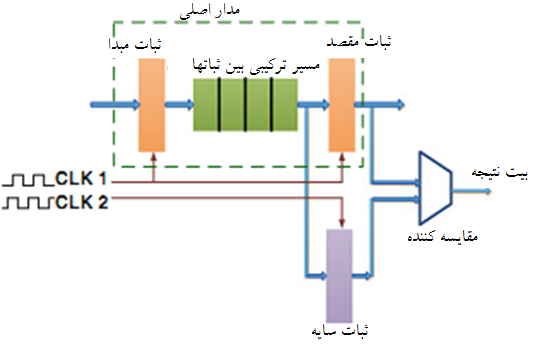
\includegraphics[scale=1]{figs/fig1-5.png}
		\caption[معماری پایه محاسبه تاخیر مسیرهای داخلی با استفاده از ثبات سایه]
		{معماری پایه محاسبه تاخیر مسیرهای داخلی با استفاده از ثبات سایه $\cite{jin2008hardware}$}
		\label{fig1-5}
	\end{center}
\end{figure} 
این معماری شامل یک ثبات سایه، یک مقایسه‌گر و یک ثبات نتیجه است. ثبات سایه با پالس ساعتی متفاوت با ساعت سیستم کار می‌کند. ساعت این ثبات، یک سیگنال است که از انحراف منفی در پالس ساعت سیستم حاصل می‌شود. در واقع فاز پالس ساعت ثبات سایه قابل تنظیم است. برای اندازه‌گیری تاخیر مسیرهای میانی، در ابتدا فاز ساعت سایه همان فاز ساعت سیستم است. بنابراین مقادیر درون ثبات سایه و ثبات مقصد مشابه هستند و خروجی مقایسه‌گر صفر است. سپس فاز ساعت سایه کاهش می یابد تا جایی که خروجی مقایسه‌گر یک شود و مقدار 1 در ثبات نتیجه ذخیره می‌شود. این مقادیر از طریق زنجیره پویش، خوانده می‌شوند.
معایب این روش:
1- گام تغییر فاز پالس ساعت سایه در دقت اندازه‌گیری تاخیر نقش اساسی دارد و تعیین کننده کارایی این روش است. استفاده از تولیدکننده سیگنال با دقت بالا نیز مساحت و توان مصرفی زیادی را تحمیل می‌کند.
2- وجود تغییرات فرآیند و نویز اندازه‌گیری می‌تواند دقت نتایج را کم کند. راه حل رایج حل این مشکل، استفاده از تحلیل داده آماری برای حذف اثر این دو است.
3- با افزایش ابعاد مدار اصلی، تعداد مسیرهای داخلی نیز افزایش یافته و بردارهای آزمون بیشتری برای پوشش این مسیرها و بهبود پوشش آزمون، باید اعمال شود. این امر هزینه را بالا می برد. 
4- هرچه تعداد مسیرهای داخلی بیشتر شود، ثبات‌های سایه بیشتری نیاز است و شبکه سیگنال ساعت ثبات‌های سایه باید گسترده تر شود. بنابراین هم سربار مساحت خواهیم داشت و هم کارایی ممکن است کاهش یابد.
\subsubsection {روش استفاده از نوسانگرهای حلقوی}
به منظور کاهش هزینه آزمون روش ثبات‌های سایه، در عین استفاده از تاخیر مسیرها، بعضی محققان به این فکر افتاده‌اند که بجای اندازه‌گیری مسیرهای موجود، مسیرهای جدیدی ایجاد کنند و تاخیر آنها را اندازه‌گیری کنند. روش استفاده از نوسانگرهای حلقوی از رایج ترین این روش‌هاست
$\cite{rajendran2011design, zhang2013detection}$. 
چرا که مساحت آنها بسیار کمتر از سایر معماری‌های بازدارنده از تروا است و از طرفی از آنجا که معماری نوسانگر حلقوی بسیار ساده است، درج آنها اثر بسیار کمی بر طراحی اولیه می‌گذارد.
شکل \ref{fig2-5} یک مدار نوسانگر حلقوی ساده را نشان می‌دهد. استفاده از دروازه‌های NAND به جای NOT کنترل‌پذیری نوسانگر را بهبود می‌دهد. تنها وقتی هر سه سیگنال کنترلی فعال باشد، نوسان انجام می‌شود و در حالت عادی این مدار سربار توان مصرفی تحمیل نمی‌کند. علاوه بر این وجود این سیگنال‌های کنترلی باعث می‌شود طراحان تروا متوجه جزئیات مدار نشوند.
\begin{figure}
	\begin{center}
		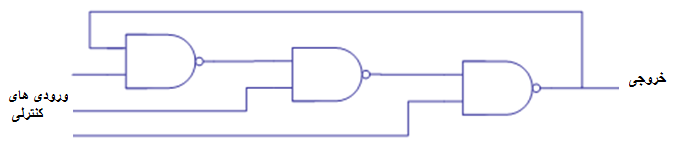
\includegraphics[scale=1]{figs/fig2-5.png}
		\caption[مدار نوسانگر حلقوی ساده]{مدار نوسانگر حلقوی ساده
			$\cite{rajendran2011design}$}
		\label{fig2-5}
	\end{center}
\end{figure} 
ایده اصلی پشت این روش، این است که هر تغییری در مدار اولیه پارامترهای نوسانگر حلقوی را نیز تغییر خواهد داد. مساله مطرح در این روش این است که چند نوسانگر باید در مدار درج شود و کجا باید اینکار انجام شود؟
روش دیگری که از ایده نوسانگرهای حلقوی استفاده می‌کند، به جای درج این نوسانگرها در مکان‌های مختلف، با استفاده از دروازه‌های منطقیِ داخل مدار اصلی و با افزودن مالتی پلکسرها، دروازه‌های NAND و معکوس کننده‌ها‌‌، نوسانگرهای حلقوی را می سازد. این روش حساسیت روش تشخیص تروا را بیشتر می‌کند. در بدترین حالت اضافه کردن مدار تروا ممکن است نوسانگر را خاموش کند.
وقتی مدار کوچک باشد، ساختن نوسانگرهای حلقوی ساده است. اما برای مدارهای پیچیده‌تر طراحان باید از الگوریتم‌هایی استفاده کنند که فرآیند درج نوسانگرها را خودکار انجام دهند. مساله دیگر نحوه محاسبه و اندازه‌گیری فرکانس نوسانگرهاست که به عنوان نشانه‌ای از تغییر تاخیر مسیرها مدنظر قرار می گیرد. اغلب برای اینکار از ماژول‌های اندازه‌گیری فرکانس روی خود تراشه استفاده می‌شود. شکل \ref{fig3-5} یک نمونه از این ماژول‌ها را نشان می‌دهد.
\begin{figure}
	\begin{center}
		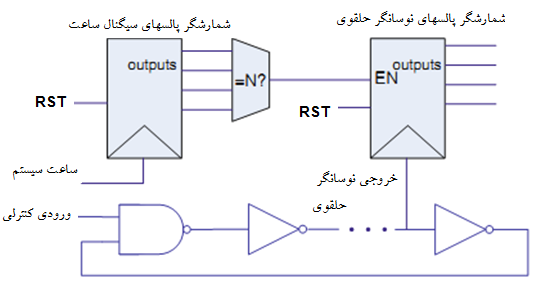
\includegraphics[scale=1]{figs/fig3-5.png}
		\caption[پیمانه اندازه‌گیری فرکانس]
		{پیمانه اندازه‌گیری فرکانس
			$\cite{zhang2013detection}$}
		\label{fig3-5}
	\end{center}
\end{figure} 
با شروع به کار مدار هر دو شمارنده شروع به شمارش می‌کنند. اولی با فرکانس مدار و دومی با فرکانس نوسانگر حلقوی. وقتی خروجی شمارنده اول برابر N شود، شمارنده دوم از کار می افتد و نسبت خروجی این شمارنده‌ها نشان دهنده فرکانس نوسانگر است. این روش سربار مساحت و توان مصرفی را افزایش می‌دهد.
\subsection {روش‌های مبتنی بر حذف رخدادهای نادر}
در $\cite{wolff2008towards}$ با فرض اینکه طراح تروا صرفاً از رخدادهای نادر برای تحریک تروا استفاده می‌کند، ایده بردارهای تروا را ارائه کرده‌اند. این بردارها رخدادهای با فرکانس پایین را تحریک می‌کنند تا بدین وسیله قابلیت تشخیص در روش‌های آزمون ساختاری قبلی، بهبود یابد. روش مبهم سازی طراحی $\cite{chakraborty2009security}$، فلیپ فلاپ‌های پویش $\cite{salmani2009new}$ و روش معکوس سازی ولتاژ $\cite{banga2009vitamin}$، همگی بر این فرضیه استوار هستند و روش‌های بازدارنده ساختاری/عملکردی محسوب می‌شوند.
مبهم سازی طراحی به معنی این است که طراحی به نحوی تغییر داده شود که از نظر عملیاتی مشابه طرح اولیه باشد ولی فهم منطق درون آن برای طراح تروا سخت‌تر باشد. بطوری که مهندسی معکوس طرح بسیار مشکل‌تر شود. در $\cite{chakraborty2009security}$ روشی برای بازدارندگی از تروا ارائه شده‌است و ماشین حالات مدار و گذار بین حالات به نحوی تغییر داده شده‌است که یک حالت مبهم‌سازی‌شده در سطحی بالاتر از عملیات اصلی (حالت عادی) مدار تعریف شود. شکل \ref{fig4-5} عملیات مبهم‌سازی‌شده و عملیات عادی را نشان می‌دهد. تنها راه رفتن از حالات مبهم‌سازی‌شده به حالات عادی، کلید K3 است.
\begin{figure}
	\begin{center}
		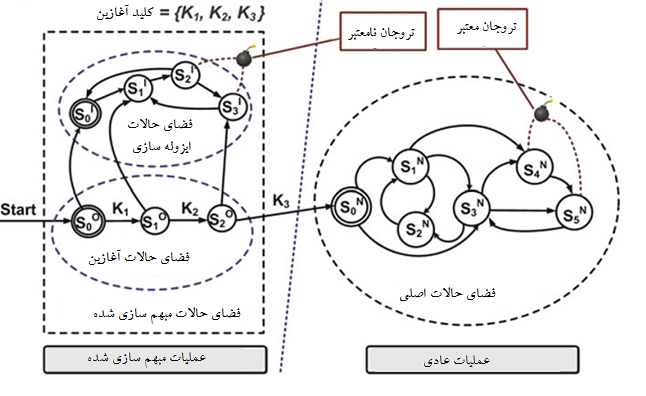
\includegraphics[scale=1]{figs/fig4-5.png}
		\caption[مدار مبهم‌سازی‌شده که شامل مدار اصلی می باشد]
		{مدار مبهم‌سازی‌شده که شامل مدار اصلی می باشد $\cite{chakraborty2009security}$}
		\label{fig4-5}
	\end{center}
\end{figure} 

الگوی ورودی که باعث گذار از حالات مبهم‌سازی‌شده به حالات عادی می‌شود را رشته کلید آغازین می‌گویند. بدون دانستن این کلید، احتمال نفوذ حمله‌کننده به حالت عمکردی عادی، بسیار کم می‌شود. بنابراین تحلیل احتمال بروز رخدادها توسط طراح تروا، اطلاعات غلطی را به وی خواهد داد. برای آنکه احتمال یافتن کلید را کاهش دهیم، باید فضای حالات مبهم‌سازی‌شده بسیار بزرگ شود. تروا‌هایی که بعد از مبهم‌سازی طراحی به آن اضافه می‌شوند، به دو دسته تقسیم می‌شوند. دسته اول تروا‌هایی هستند که همه یا بخشی از مدار تحریکشان شامل حالات داخل بخش مبهم‌سازی‌شده ‌است و دسته دوم آنهایی هستند که تمام مدار تحریکشان شامل حالات بخش عادی مدار است. تروا‌های دسته اول در حالت عادی، به هیچ وجه تحریک نمی‌شوند و نگرانی درباره آنها نداریم. اما تروا‌های دسته دوم ممکن است تحریک شوند. اما به علت اینکه احتمالاتی که طراح تروا از شبیه‌سازی‌ها بدست آورده، ارقام اشتباهی بوده است، لزوماً مدار تحریک این تروا‌ها شامل رخدادهای نادر نخواهد بود. برای پیاده‌سازی مبهم‌سازی طراحی، می‌توان از ابزارهای طراحی خودکار استفاده کرد. برای خودکارسازی این کار، الگوریتمی در $\cite{chakraborty2009security}$ ارائه شده‌است.
معایب این روش:
در بسیاری از موارد، فرضیات این روش صحیح نخواهد بود. اولین فرض این است که طراح تروا تنها از رخدادهای نادر برای تحریک تروا استفاده می‌کند. این در حالیست که اولاً برخی از تروا‌ها همیشه فعال هستند. ثانیاً تعریف نادر بودن یک رخداد ممکن است از دید طراح سیستم و طراح تروا متفاوت باشد. فرض دوم این روش این است که طراح تروا هیچ دیدی نسبت به نحوه مبهم‌سازی طراحی ندارد. اگر هریک از این فرضیات درست نباشد، کارایی این روش کاهش خواهد یافت.
در $\cite{salmani2009new}$ احتمال گذار سیم‌های داخلی با یک توزیع هندسی مدل شده‌است و روش بازدارنده از تروای ارائه شده‌است که می‌تواند احتمال گذار مدارات تروا عملیاتی را افزایش دهد. برای این کار، فلیپ فلاپ‌های اضافی با نام فلیپ فلاپ‌های ساختگی، به مدار اضافه می‌شوند به نحوی که عملکرد مدار را تغییر ندهند. شکل \ref{fig5-5} مدار اصلی و مدار شامل فلیپ فلاپ‌های ساختگی را نشان می‌دهد. همانطور که در شکل نشان داده شده‌است، احتمال یک شدن خروجی مدار با این روش 8.5 برابر شده‌است.
\begin{figure}
	\begin{center}
		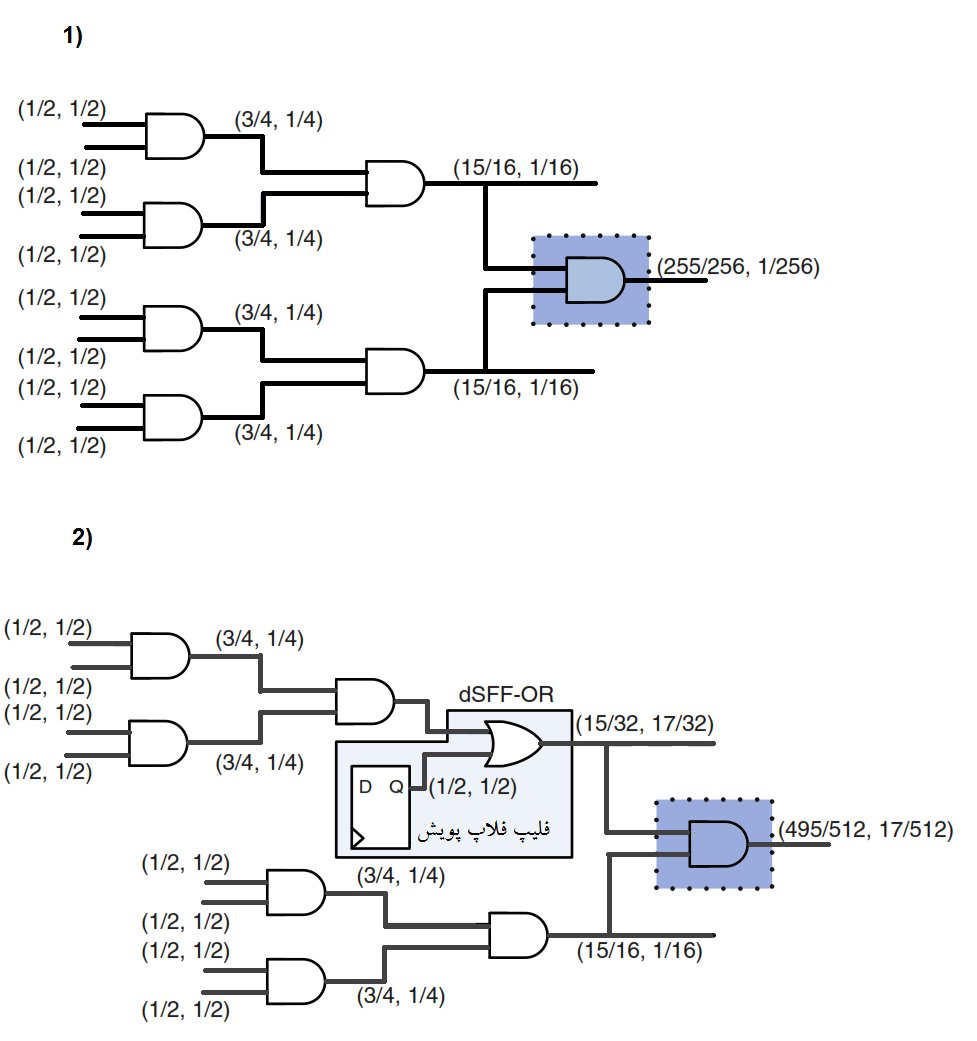
\includegraphics[scale=0.6]{figs/fig5-5.png}
		\caption[مدار اصلی و مدار شامل فلیپ فلاپ‌های ساختگی]{مدار اصلی و مدار شامل فلیپ فلاپ‌های ساختگی
			$\cite{salmani2009new}$}
		\label{fig5-5}
	\end{center}
\end{figure} 
این روش از دو طریق می‌تواند به تشخیص تروا و بازدارندگی از تروا کمک کند:
1- تحلیل اثرات جانبی مبتنی بر توان مصرفی:
به علت اضافه کردن فلیپ فلاپ‌ها و دروازه‌های منطقی مربوط به آنها به مدار ، فعالیت تروا در حالت آزمون بیشتر خواهد شد و توان بیشتری مصرف خواهد کرد. 
2- آزمون عملیاتی:
فلیپ فلاپ‌های اضافه می‌توانند احتمال گذار سیم‌های داخلی را به نحوی تعدیل کنند که احتمال فعال شدن تروا افزایش یابد. بنابراین فرضیه رخداد نادر که طراح تروا طرح خود را بر آن استوار کرده‌است، صحیح نخواهد بود و در طول فاز آزمون نتایج غلط در خروجی‌ها مشاهده خواهد شد.
در $\cite{banga2009vitamin}$ یک روش وارونه‌سازی ولتاژ برای افزایش فعالیت تروا بدون افزودن دروازه‌های منطقی اضافه، ارائه شده‌است. ایده اصلی این است که با جابجا کردن تغذیه و زمین در دروازه‌های منطقی، عملکرد آن به نحوی تغییر می‌کند که خروجیِ با احتمال کم، بیشتر رخ خواهد داد. 
در منطق CMOS، وارونه کردن ولتاژ تغذیه باعث کاهش پتانسیل دروازه منطقی می‌شود و این امر باعث می‌شود پتانسیل طبقات بعدی نیز کاهش یابد. این امر باعث می‌شود بعد از چند طبقه، دیگر سیگنال در مدار منتشر نشود. برای جلوگیری از این امر نیز در این مقاله راهکاری ارائه شده‌است.
در $\cite{abramovici2009integrated}$ منطق زیرساختی برای انجام بررسی‌های امنیتیِ برخط در طول عملکرد عادی مدار، ارائه شده‌است که متمرکز بر حوزه SoC است. مدار با قابلیت بازپیکربندی موسوم به DEFENSE که مخفف «طراحی برای امنیت» است، به SoC افزوده می‌شود تا نظارت بر ناهنجاری‌ها را در زمان اجرا انجام دهد. شکل \ref{fig6-5} معماری چنین SoC ای را نشان می‌دهد.
\begin{figure}
	\begin{center}
		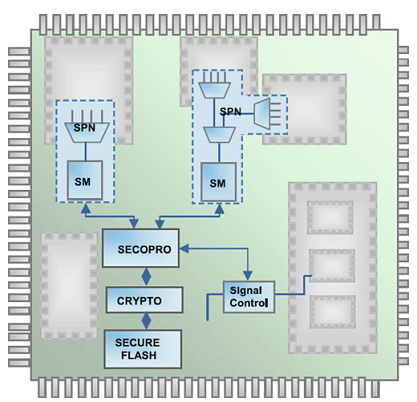
\includegraphics[scale=0.6]{figs/fig6-5.png}
		\caption[معماری SoC شامل پیمانه‌های DEFENSE]
		{معماری SoC شامل پیمانه‌های DEFENSE
			$\cite{abramovici2009integrated}$}
		\label{fig6-5}
	\end{center}
\end{figure} 
پیمانه اصلی این زیرساخت، زوج مدار SPN یا شبکه پویش سیگنال و SM یا ناظر امنیت است. SPN که شبکه ای از مالتی پلکسرهای توزیع شده‌است، به نحوی پیکربندی می‌شود که زیرمجموعه‌ای از سیگنال‌های مهم تعریف شده توسط کاربر را انتخاب کند و به واحد SM منتقل کند. در این واحد رفتار مورد انتظار کاربر بررسی می‌شود. پردازشگر امنیت و کنترل SECOPRO به نحوی SPN را پیکربندی می‌کند که به طور پویا سیگنال‌های لازم را انتخاب کند. این پیکربندی‌ها رمز شده و در یک حافظه امن نگهداری می‌شود. وقتی ناهنجاری رفتاری تشخیص داده شود، پیمانه کنترل سیگنال SECOPRO را فعال می‌کند تا مقادیر سیگنال‌های مشکوک را بازنویسی کند و سیستم را به حالت عادی برگرداند. همچنین، هسته‌ای که رفتار نادرست داشته است، کنار گذاشته می‌شود. 
معایب این روش:
سربار سخت‌افزاری ناشی از پیمانه‌های این زیرساخت مساله قابل تاملی است.
\subsection {طراحی برای آزمون تروا}
در $\cite{jin2010dftt}$ یک روش مقاوم سازی سخت‌افزار در برابر تروا ارائه شده‌است که مشابه روش مرسوم طراحی برای آزمون (DFT) در آزمون اشکال است. از آنجا که هدف این روش، مقاوم سازی دربرابر تروا است، طراحی برای آزمون تروا نام گرفته‌است. البته علیرغم شباهت در نام، تفاوت‌های بسیاری بین DFT و DFTT وجود دارد. هدف DFT یافتن اشکالات داخل مدار بدون تروا با ایجاد بردارهای آزمون است. در حالیکه هدف DFTT تشخیص حضور یا عدم حضور تروا با استفاده از این بردارهاست. در شکل \ref{fig7-5} سه گام اصلی این روش که در ادامه توضیح داده می‌شود، نشان داده شده‌است.
\begin{figure}
	\begin{center}
		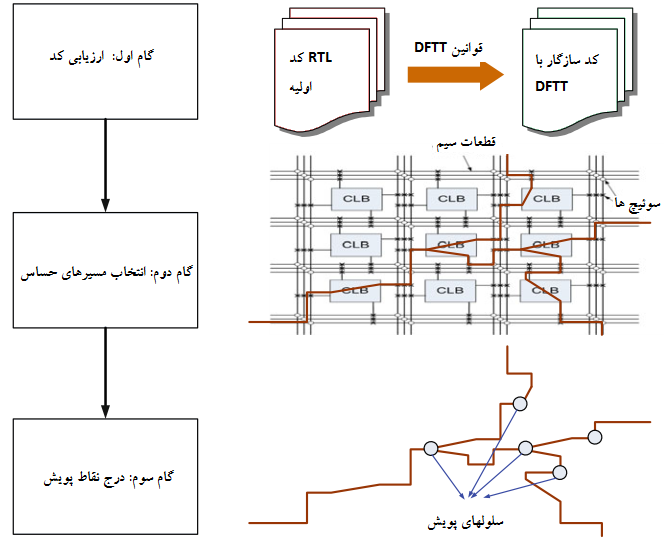
\includegraphics[scale=1]{figs/fig7-5.png}
		\caption[گامهای اصلی در روشDFTT]
		{گامهای اصلی در روشDFTT $\cite{jin2010dftt}$}
		\label{fig7-5}
	\end{center}
\end{figure} 
گام اول: ارزیابی کد:
کد HDL مربوط به مدار اصلی با استفاده از قوانین کد نویسی DFTT به یک کد سازگار با DFTT تبدیل می‌شود.
گام دوم: انتخاب مسیرهای حساس:
فرض بر این است که طراحان تروا قصد دارند مداری به مدار اصلی اضافه کنند که از طریق آن اطلاعات حساس داخلی را سرقت کنند. بدین منظور قبل از درج تروا، تلاش می‌کنند تا اهمیت نسبی سیگنال‌های داخلی(مانند کلید رمز در مدارات رمز نگاری) را ارزیابی کنند. بنابراین ابزار DFTT که برای خودکار سازی عملیات DFTT طراحی شده‌است، مسیرهایی را که سیگنال‌های حساس از آنها عبور می‌کنند یا به عملکرد سیگنال‌های حساس مدد می‌رسانند، به نحوی از مسیر بین ورودی‌های مدار تا خروجی‌های مدار برکنار می دارد.
گام سوم: درج نقاط پویش:
براساس مسیرهای حساسی که در گام دوم انتخاب شد، سلولهای پویش در کد سازگار با DFTT درج می‌شود. این گام مشابه درج فلیپ فلاپ‌های پویش در هنگام استفاده از DFT است. اما سلولهای پویش کمی متفاوت هستند. 
بعد از اینکه طراحی ما با این روش مقاوم سازی شد، بقیه مراحل آزمون مشابه DFT است.
\subsection {سخت‌افزار حامل اثبات}
در $\cite{hsiaotrust}$ نویسندگان تلاش کرده‌اند محدودیت روش‌های تشخیص تروا رایج را بیان کنند. اینکه همه این روش‌ها سعی در بررسی حضور تروا در تراشه‌های ساخته شده دارند. اما درباره بررسی حضور تروا در طرح، قبل از ساخت آن، تلاش اندکی انجام شده‌است. روش‌هایی که تا کنون برای طراحی سخت‌افزار مطمئن معرفی شدند، هیچکدام تلاشی برای حفاظت از IP‌ها‌‌ی سخت‌افزاری در برابر تروا نکرده‌اند. درمورد IP‌ها‌‌ی نرم‌افزاری در سال 1996 روش PCC یا کد حامل اثبات، ارائه شده‌است. در این روش یک اثبات سوری که به صورت خودکار قابل صحت سنجی است، تعیین می‌کند که آیا کد مورد نظر از یک سری ویژگی‌های سوری پیروی می‌کند یا نه. بعد از آن، این اثبات با کد ترکیب می‌شود تا گیرنده بتواند به طور خودکار کد را نسبت به اثبات چک کند و تصمیم بگیرد که کد را اجرا کند یا نه.
ایده گسترش این روش به حوزه سخت‌افزار مطمئن اولین بار در $\cite{drzevitzky2009proof}$ مطرح شد. نویسندگان این مقاله با اشاره به گسترش استفاده از FPGA‌ها‌‌ و ابزارهای قابل بازپیکربندی، بر لزوم ارائه روش PCH تاکید کرده‌اند. به عنوان اولین گام در امنیت سخت‌افزار قابل اثبات، نویسندگان این مقاله روشی ارائه کرده‌اند که اثبات‌های مربوط به یکسانی مدارهای ترکیبی پیاده‌سازی شده در FPGA را فراهم می‌کند. این روش نیازمند یک تابع مشخصه S(x) برای هر عملیات منطقی و یک پیاده‌سازی I(x) استخراج شده از netlist مربوط به FPGA است. با این دو ورودی، اثبات به طور خودکار برای نشان دادن یکسانی S(x) با I(x) تولید می‌شود. نویسندگان این مقاله ساختاری به نام miter ایجاد کرده‌اند که از اعمال تابع XOR روی S(x) و I(x) حاصل شده‌است. هنگامی خروجی miter درست می‌شود که به ازای یک x این دو با یکدیگر نامساوی باشند. بنابراین اگر miter به هیچ وجه درست نباشد، یعنی مشخصه با پیاده‌سازی برابر است. محدودیت این روش این است که باید تابع بولی معادل مدار را داشته باشیم.
در $\cite{love2011enhancing}$ برای رفع محدودیت روش PCH ، PCHIP را برای ضمانت اثبات‌های مربوط به کد HDL مدار به جای رشته بیتی FPGA ارائه کرده‌اند. در این روش یک پروتکل جدید برای طراحی هسته‌های IP سخت‌افزاری ارائه شده‌است که در \ref{fig8-5} نشان داده شده‌است.
\begin{figure}
	\begin{center}
		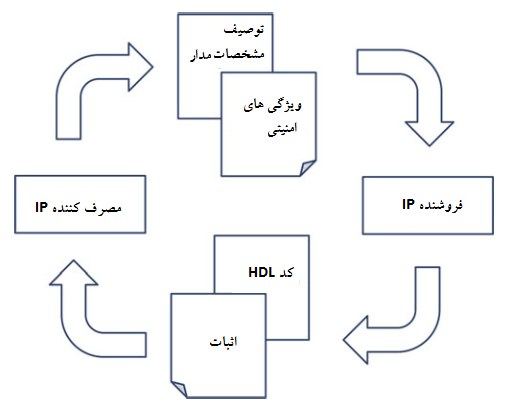
\includegraphics[scale=.8]{figs/fig8-5.png}
		\caption[روند طراحی هسته‌های IP و تولید و بررسی اثبات در روش PCHIP]
		{روند طراحی هسته‌های IP و تولید و بررسی اثبات در روش PCHIP $\cite{love2011enhancing}$}
		\label{fig8-5}
	\end{center}
\end{figure} 

\subsection{مقایسه روش‌های تشخیص تروا} 
\subsubsection{ مقایسه رویکردهای تشخیص تروا بر اساس اندازه نسبی تروا}
جدول زیر خلاصه ای از مزایا و معایب نسبی روش‌های مبتنی بر آزمون منطقی را در مقایسه با روش‌های مبتنی بر تحلیل اثرات جانبی برای تشخیص تروا نشان می‌دهد. واضح است که دو روش مکمل یکدیگر هستند. بنابراین رویکردهایی که نقاط قوت هر دو را ترکیب کنند، می‌توانند مورد توجه بیشتری قرار گیرند. مزیت اصلی روش‌های زمان آزمون، عدم وجود سربار سخت‌افزاری است. درحالیکه عیب اصلی آنها نیازمندی به یک مدار مرجع یا مدار بدون تروا برای انجام مقایسه‌هاست. روش‌های زمان اجرا معمولاً سربار کارایی و توان مصرفی بالایی دارند ولی در مقابل امکان ایجاد اطمینان 100\% را فراهم می‌کنند. 
\begin{table}[t]
	\label{tcomparisonls}
	\caption{مقایسه آزمون‌های منطقی و اثرات جانبی}
	\begin{center}
		\begin{tabular}{| p{4cm} | p{4cm} || c |}
			\hline
			\textbf{رویکرد تحلیل اثرات جانبی} & \textbf{رویکرد آزمون منطقی} & \\ \hline \hline
			برای تروا‌های بزرگ موثر است تولید بردارهای آزمون ساده است & برای تروا‌های کوچک موثر است درمقابل نویز فرآیند تاثیرپذیر نیست &\textbf{ مزایا} \\ \hline
			نسبت به نویز فرآیند حساس است تشخیص تروا‌های کوچک مساله ساز است & تولید بردارهای آزمون پیچیده است. تشخیص تروا‌های بزرگ مساله ساز است & \textbf{معایب} \\ \hline
		\end{tabular}
	\end{center}
\end{table}
\subsubsection{بررسی و مقایسه روش‌های تشخیص تروا}

در این بخش برخی از روش‌های تشخیص تروا حین آزمون شرح داده می‌شود و مزایا و معایب نسبی آنها مقایسه می‌شود. اکثر روش‌های تشخیص تروا که تا کنون ارائه شده‌است، در این دسته قرار می‌گیرند. برخی از این روش‌ها از روش آزمون عملکردی استفاده می‌کنند و برخی دیگر اثرات جانبی را تحلیل می‌کنند.
%
\begin{table}
	\caption{مقایسه روش‌های مقابله با تروا}
	\label{tcomparison}
	\begin{tabular}{|p{1cm}||p{3cm}|p{3cm}|p{3cm}|p{3cm}|}
		\hline

		نوع روش & نام روش  & تروا‌های قابل ئشخیص & سربار& معایب دیگر \\ \hline \hline
		روش ‌های آزمون منطقی& روش تولید بردارهای آزمون&اغلب تروا‌های با تحریک ترکیبی، تعداد معدودی از تروا‌های با تحریک ترتیبی(  فقط تروا‌هایی که با شرایط خاص فعال می‌شوند)&این روش در حین آزمون انجام می‌شود و سربار زمانی بسیار زیادی دارد.(44.5 ساعت برای مدار c7552 )&طبق نتایج مقاله، پوشش دهی تروا‌ها برای مدارهای ترتیبی نسبت به روش بردارهای تصادفی تفاوت چندانی نداشته و در برخی موارد کمتر شده‌است. ضمن اینکه  این روش نیاز به تحلیل قبلی مدار برای یافتن رخدادهای نادر دارد.
		
		MERO [27]
		
		\\ \cline{2-5}
		&روش شفاف کردن ماژول­ها (افزایش کنترل پذیری و مشاهده پذیری) [29]  &فقط تروا‌های خیلی بزرگ ( فقط تروا‌هایی که در شرایط خاص فعال می‌شوند)&طبق گزارش مقاله 5\% سربار مساحت، 13\% سربار توان مصرفی، 5\% سربار تاخیر و 9 پایه اضافه لازم است. & نحوه اعمال کلیدها به ماژول­ها و ایجاد امضای خروجی، در نتیجه این روش موثر است که در این مقاله توضیح چندانی داده نشده‌است.
		\\ \hline \hline 
	\end{tabular}
\end{table}
\newpage
\begin{table}
	\begin{tabular}{|p{1cm}||p{3cm}|p{3cm}|p{3cm}|p{3cm}|}
		روش ‌های تحلیل اثرات جانبی با رویکرد اندازه ‌گیری توان مصرفی&روش ناحیه بندی [10]  &فقط تروا‌های با تحریک ترتیبی که در شرایط خاص فعال می‌شوند &سربار زمانی حین آزمون زیاد است و هرچه مدار بزرگتر شود، این سربار بیشتر می‌شود. &میزان نتیجه گیری کاملا وابسته به شخص است. چرا که هیچ روند خودکار­سازی برای ناحیه­بندی و ایجاد بردارهای آزمون ارائه نشده‌است. 
		%	\end{tabular}

		
		%\begin{tabular}{|p{1cm}||p{3cm}|p{3cm}|p{3cm}|p{3cm}|}

		\\ \cline{2-5}
		&روش اعمال بردارهای پایدار شده [24]  &اغلب تروا‌های با تحریک ترکیبی، تعداد معدودی از تروا‌های با تحریک ترتیبی ( فقط تروا‌هایی که با شرایط خاص فعال می‌شوند)  &سربار زمانی زیاد در حین آزمون به علت ثابت نگهداشتن بردار ورودی برای مدت زمان تعیین شده لازم ‌است. &افزایش حرارت و در پی آن کاهش عمر مدار به علت افزایش خودخواسته توان مصرفی
		
		\\ \cline{2-5}
		& روش محاسبه جریان از طریق پایه­های تغذیه مختلف [6] &این روش فقط برای یک مدار ترکیبی آزموده شده‌است. برای مدارات ترتیبی خیلی مناسب نخواهد بود. & سربار ابزارهای جانبی اندازه‌گیری دقیق جریان - سربار زمانی حین آزمون&پوشش تروا پایین در حد 50\% برای تروا‌های فعال و 30\% برای تروا‌های غیرفعال 
		\\ \cline{2-5}
		& استفاده از ترتیب دهی مجدد فلیپ فلاپ‌های پویش [16] &انواع تروا‌های کوچک و بزرگ (فقط تروا‌هایی که با شرایط خاص فعال می‌شوند)  &سربار زمانی حین آزمون & عدم تشخیص برخی تروا‌های با تحریک ترتیبی- نیاز به پایه­های اضافه برای تراشه، بسته به کوچکترین تروا قابل تشخیص
		\\ \hline \hline
		
		روش ‌های تحلیل اثرات جانبی با رویکرد اندازه ‌گیری تاخیر& محاسبه تاخیر مسیرها [7] & فقط تروا‌های با تحریک ترکیبی- تشخیص تروا‌های بزرگ راحت تر است.& سربار زمانی حین آزمون&عدم تشخیص تروا‌هایی که در مسیر بین ورودی و خروجی مدار واقع نشده و در مسیرهای داخلی اند.
		\\ \cline{2-5}
		%\end{tabular}

		
		
		%\begin{tabular}{|p{1cm}||p{3cm}|p{3cm}|p{3cm}|p{3cm}|}

		&محاسبه تاخیر مسیرهای داخلی با استفاده از ثبات‌های سایه [8]  &انواع تروا‌ها با اولویت تروا‌های بزرگ (هرچه اندازه تروا‌ها کوچکتر باشد، نیاز به سربار بیشتر زمانی و پیچیدگی بیشتر طراحی است) &سربار زمانی زیاد حین آزمون- سربار مساحت و توان ناشی از تولید کننده سیگنال کلاک – سربار مساحت و توان ثبات‌های سایه &دقت تشخیص تروا وابسته به گام تغییر فاز کلاک است که پیچیدگی را زیاد می­کند. با افزایش ابعاد مدار شبکه توزیع کلاک دردسرساز می‌شود.
		\\ \hline \hline
		&تشخیص تغییرات تاخیر با استفاده از نوسانگرهای حلقوی [30,31]&فقط تروا‌های با تحریک ترکیبی- تشخیص تروا‌های بزرگ راحت تر است.&سربار مساحت و توان نوسانگرها یا مدارات اضافه جهت ساختن آنها در مدار-  سربار زمانی حین آزمون برای خواندن نتایج- سربار مساحت و توان اندازه گیرهای فرکانس&تعداد نوسانگرها و موقعیت درج آنها کاملا وابسته به دانش فرد طراح است.
		\\ \hline
	\end{tabular}
	
\end{table}

\begin{table}
	\label{tcomparison}
	\begin{tabular}{|p{1cm}||p{3cm}|p{3cm}|p{3cm}|p{3cm}|}
		\hline
		
		نوع روش & نام روش & تروا‌های قابل ئشخیص & سربار& معایب دیگر \\ \hline \hline
		روش‌ها‌‌ی آزمون منطقی& روش تولید بردارهای آزمون&اغلب تروا‌های با تحریک ترکیبی، تعداد معدودی از تروا‌های با تحریک ترتیبی( فقط تروا‌هایی که با شرایط خاص فعال می‌شوند)&این روش در حین آزمون انجام می‌شود و سربار زمانی بسیار زیادی دارد.(44.5 ساعت برای مدار c7552 )&طبق نتایج مقاله، پوشش دهی تروا‌ها برای مدارهای ترتیبی نسبت به روش بردارهای تصادفی تفاوت چندانی نداشته و در برخی موارد کمتر شده‌است. ضمن اینکه این روش نیاز به تحلیل قبلی مدار برای یافتن رخدادهای نادر دارد.
		MERO $\cite{torrance2007reverse}$
		\\ \cline{2-5}
		&روش شفاف کردن پیمانه‌ها (افزایش کنترل پذیری و مشاهده پذیری) $\cite{aarestad2010detecting}$ &فقط تروا‌های خیلی بزرگ ( فقط تروا‌هایی که در شرایط خاص فعال می‌شوند)&طبق گزارش مقاله $5\% $ سربار مساحت، $ 13\%$ سربار توان مصرفی، $5\%$ سربار تاخیر و 9 پایه اضافه لازم است. & نحوه اعمال کلیدها به پیمانه‌‌ها و ایجاد امضای خروجی، در نتیجه این روش موثر است که در این مقاله توضیح چندانی داده نشده‌است.
		
	\end{tabular}
\end{table}
\newpage
\begin{table}
	\begin{tabular}{|p{1cm}||p{3cm}|p{3cm}|p{3cm}|p{3cm}|}
		نوع روش & نام روش & تروا‌های قابل ئشخیص & سربار& معایب دیگر \\ \hline \hline
		روش‌ها‌‌ی تحلیل اثرات جانبی با رویکرد اندازه ‌گیری توان مصرفی&روش ناحیه بندی $\cite{banga2008region}$ &فقط تروا‌های با تحریک ترتیبی که در شرایط خاص فعال می‌شوند &سربار زمانی حین آزمون زیاد است و هرچه مدار بزرگتر شود، این سربار بیشتر می‌شود. &میزان نتیجه گیری کاملا وابسته به شخص است. چرا که هیچ روند خودکار‌‌سازی برای ناحیه‌‌بندی و ایجاد بردارهای آزمون ارائه نشده‌است. 
		% \end{tabular}
		
		%\begin{tabular}{|p{1cm}||p{3cm}|p{3cm}|p{3cm}|p{3cm}|}
		
		\\ \cline{2-5}
		&روش اعمال بردارهای پایدار شده $\cite{chakraborty2009hardware}$ &اغلب تروا‌های با تحریک ترکیبی، تعداد معدودی از تروا‌های با تحریک ترتیبی ( فقط تروا‌هایی که با شرایط خاص فعال می‌شوند) &سربار زمانی زیاد در حین آزمون به علت ثابت نگهداشتن بردار ورودی برای مدت زمان تعیین شده لازم ‌است. &افزایش حرارت و در پی آن کاهش عمر مدار به علت افزایش خودخواسته توان مصرفی
		\\ \cline{2-5}
		& روش محاسبه جریان از طریق پایه‌‌های تغذیه مختلف $\cite{wang2008hardware}$ &این روش فقط برای یک مدار ترکیبی آزموده شده‌است. برای مدارات ترتیبی خیلی مناسب نخواهد بود. & سربار ابزارهای جانبی اندازه‌گیری دقیق جریان - سربار زمانی حین آزمون&پوشش تروا پایین در حد $50\%$ برای تروا‌های فعال و $ 30\%$ برای تروا‌های غیرفعال 
	\end{tabular}
\end{table}
\newpage
\begin{table}
	\begin{tabular}{|p{1cm}||p{3cm}|p{3cm}|p{3cm}|p{3cm}|}
		نوع روش & نام روش & تروا‌های قابل ئشخیص & سربار& معایب دیگر \\ \hline \hline
		& استفاده از ترتیب دهی مجدد فلیپ فلاپ‌های پویش $\cite{salmani2009new}$ &انواع تروا‌های کوچک و بزرگ (فقط تروا‌هایی که با شرایط خاص فعال می‌شوند) &سربار زمانی حین آزمون & عدم تشخیص برخی تروا‌های با تحریک ترتیبی- نیاز به پایه‌‌های اضافه برای تراشه، بسته به کوچکترین تروا قابل تشخیص
		\\ \hline \hline
		روش‌ها‌‌ی تحلیل اثرات جانبی با رویکرد اندازه ‌گیری تاخیر& محاسبه تاخیر مسیرها $\cite{jin2008hardware}$ & فقط تروا‌های با تحریک ترکیبی- تشخیص تروا‌های بزرگ راحت تر است.& سربار زمانی حین آزمون&عدم تشخیص تروا‌هایی که در مسیر بین ورودی و خروجی مدار واقع نشده و در مسیرهای داخلی اند.
		\\ \cline{2-5}
		%\end{tabular}
		
		%\begin{tabular}{|p{1cm}||p{3cm}|p{3cm}|p{3cm}|p{3cm}|}
		
		&محاسبه تاخیر مسیرهای داخلی با استفاده از ثبات‌های سایه $\cite{li2008speed}$ &انواع تروا‌ها با اولویت تروا‌های بزرگ (هرچه اندازه تروا‌ها کوچکتر باشد، نیاز به سربار بیشتر زمانی و پیچیدگی بیشتر طراحی است) &سربار زمانی زیاد حین آزمون- سربار مساحت و توان ناشی از تولید کننده سیگنال کلاک – سربار مساحت و توان ثبات‌های سایه &دقت تشخیص تروا وابسته به گام تغییر فاز کلاک است که پیچیدگی را زیاد می‌‌کند. با افزایش ابعاد مدار شبکه توزیع کلاک دردسرساز می‌شود.
	\end{tabular}
\end{table}
\newpage
\begin{table}
	\begin{tabular}{|p{1cm}||p{3cm}|p{3cm}|p{3cm}|p{3cm}|}
		نوع روش & نام روش & تروا‌های قابل ئشخیص & سربار& معایب دیگر \\ \hline \hline
		&تشخیص تغییرات تاخیر با استفاده از نوسانگرهای حلقوی
		$\cite{alkabani2009consistency, potkonjak2009hardware}$
		&فقط تروا‌های با تحریک ترکیبی- تشخیص تروا‌های بزرگ راحت تر است.&سربار مساحت و توان نوسانگرها یا مدارات اضافه جهت ساختن آنها در مدار- سربار زمانی حین آزمون برای خواندن نتایج- سربار مساحت و توان اندازه گیرهای فرکانس&تعداد نوسانگرها و موقعیت درج آنها کاملا وابسته به دانش فرد طراح است.
		\\ \hline \hline
	\end{tabular}
	\caption{مقایسه روش‌های مقابله با تروا}
\end{table}


